\section{Diffusion models}\label{diffusion Models}

Diffusion models have emerged as a prominent method in generative modeling, offering distinct advantages over traditional models like Variational Autoencoders (VAEs) and Generative Adversarial Networks (GANs). They operate by progressively perturbing data with noise and then learning to reverse this process, a methodology that enables the generation of highly realistic and diverse new samples.

~\cite{yangdiffusionSummary} distinguish between three main approaches that dominate the study of diffusion models, which are going to be discussed shortly: Denoising Diffusion Probabilistic Models (DDPMs) \citep{hoDDPMs,sohlDDPM}, Score-based Generative Models (SGMs) \citep{song2019SGM}, and Stochastic Differential Equations (Score SDEs) \citep{song2020score, song2021maximum}. Each of these models has its own set of strengths and challenges, contributing uniquely to the development of Diffusion Models.

\subsection{Denoising Diffusion Probabilistic Models}\label{DDPMs}

Central to the concept of Denoising Diffusion Probabilistic Models (DDPMs) are two Markov chains: the forward chain and the reverse chain, also known as the forward and reverse diffusion processes \citep{sohlDDPM}.

The forward diffusion process, sharing some similarities with VAEs, focuses on a latent feature space of the initial data distribution. However, DDPMs differ in that the forward process in DDPMs ``is fixed to a Markov chain that gradually [over a span of T steps] adds Gaussian noise to the data according to a variance schedule \(\beta_1, \ldots, \beta_T \)''~\cite{hoDDPMs}. This process gradually pertubes the data's structure, eventually resulting in an image of pure noise, with the aim of gradually steering the data distribution towards a more manageable prior distribution \citep{yangdiffusionSummary, pooleDreamfusion}. 

The mathematical formulation of the forward process is given by \citeauthor{martinez2023understanding}:

\[
q(x_t | x_{t-1}) = \mathcal{N}(x_t; \sqrt{1 - \beta_t}x_{t-1}, \beta_t I) \quad \text{where} \quad \sqrt{1 - \beta_t}x_{t-1} = \mu_t \quad \text{and} \quad \beta_t I = \Sigma_t
\] 

In this equation, the model first adjusts the previous data point \( x_{t-1} \) to get \( x_t \), the data point at the current step. This adjustment follows a Gaussian distribution and is done using the term \( \sqrt{1 - \beta_t} x_{t-1} \), which slightly reduces the intensity or strength of the previous data point \citep{sohlDDPM, hoDDPMs}. This controlled approach helps maintain a balance between the original data and the noise, ensuring that the noise doesn't overwhelm the data too quickly. Once this preparatory step is completed, the model then introduces noise. The level of noise added at each step is determined by the parameter \( \beta_t \), where a higher value means more noise is added \citep{kingma2023variationalDM}. The way noise is added is described by the covariance matrix \( \beta_t I \), where \( I \) is the identity matrix. This matrix ensures that noise is added to each element of the data in an independent and uniform manner, evenly distributing the noise across all parts of the data. The importance of this noise-adding process lies in its role in teaching the model the structure and characteristics of noise. By gradually adding noise to the data, the model learns how images degrade step by step, knowledge that is crucial for the reverse process of DDPMs.

The process of adding noise over the entire sequence from the original data point \( x_0 \) to \( x_T \) is captured another formular by \citeauthor{martinez2023understanding}:

\[q(x_{1:T} | x_0) = \prod_{t=1}^T q(x_t | x_{t-1}) \] 

Built upon the Markov property, the formula implies that each step depends solely on the previous step, allowing for a systematic and gradual transformation from \( x_0 \) to \( x_T \) \citep{martinez2023understanding}. This methodical approach provides a detailed understanding of the data's evolution at each noise addition stage, giving a complete view of the transition probabilities throughout the forward diffusion process.

\begin{figure}[ht]
\centering
  \includegraphics[width=1\columnwidth]{figures/manta_DDMP3.png}
  \caption{Illustration of the Forward Diffusion Process in DDPMs: This figure demonstrates the gradual addition of Gaussian noise to an image over multiple steps. Each subsequent image from left to right shows an increased level of noise, culminating in the far-right image, which represents a state of pure noise.}\label{fig:figureForwardProcess}
\end{figure}

The reverse diffusion process employs a neural network parameterized by \(\Theta\), to approximate the inverse of the forward process. It estimates the prior state of data points, \( x_{t-1} \), from their current noisy state, \( x_t \), using the probability distribution function \( p_\theta(x_{t-1} | x_t) \), as given by \citeauthor{martinez2023understanding}. This process is modeled as a normal distribution where the mean \( \mu_\theta(x_t, t) \) and covariance \( \Sigma_\theta(x_t, t) \) are determined by the neural network \citep{yangdiffusionSummary}.

\[
  p_\theta(x_{t-1} | x_t) = \mathcal{N}(x_{t-1}; \mu_\theta(x_t, t), \Sigma_\theta(x_t, t))
\] 

\[p_\theta(x_{0:T}) = p_\theta(x_{T}) \prod_{t=1}^T p_\theta(x_{t-1} | x_t) \]

The latter function \(p_\theta(x_{0:T})\) is also taken from \citeauthor{martinez2023understanding} and captures the probability of the entire data sequence under the reverse process, beginning with an estimate of the final noisy data point \(p_\theta(x_{T})\) and progressively reconstructing the data by removing noise at each step \citep{hoDDPMs,martinez2023understanding}. Unlike the forward process that adds noise, the reverse process, starting from a state of random noise, uses the learned noise patterns to iteratively generate coherent images. The reverse process is also a Markov chain and involves the neural network learning to predict the reverse diffusion parameters \(\Theta\) at each timestep \citep{yangdiffusionSummary}. The goal here is to ensure that the new samples it generates are statistically similar to the original data it was trained on. This is done by maximizing the likelihood that these new samples belong to the same overall data distribution as the original set \citep{yangdiffusionSummary}.

\begin{comment}
[
In the reverse process, the neural network can be trained to predict one of three possibilities: the mean of the noise at each time step, the original image itself, or the noise of the image \citep{hoDDPMs}. The second approach is not as advantageous as the ``estimating small perturbations is easier than explicitly describing the entire distribution with a single, non-analytically normalizable potential function'' \citep{sohlDDPM}. Focusing on the prediction of image noise is preferable because it allows a simple subtraction of the noise from the image, resulting in a less noisy version and thus also allowing an iterative generation of an image from the noise.
]
\end{comment}

Despite their effectiveness, DDPMs are not without challenges. The most significant of these is the computational time required for generating new samples, which is due to ``a Markov process [that] has to be simulated at each generation step, which greatly slows down the process'' \citep{martinez2023understanding}.
\subsection{Score-Based Generative Models}\label{SGMs}

In the domain of generative modeling, Score-Based Generative Models (SGMs), as introduced by \citeauthor{song2019SGM}, distinguish themselves by prioritizing the learning of a score function using the Stein score \citep{steinScore}. The score is ``the gradient of the log-density function at the input data point'' \citep{song2019SGM}, serving as a guide towards higher data density regions. The score function is central in SGMs, akin to how DDPMs use a forward process of adding noise, but with a different purpose. In SGMs, the score guides the model to areas in the data space where the probability of finding similar data points to the training set is higher.

SGMs begin their learning process with a set of training data. Common data distributions indicate areas of high probability, while rare inputs usually result in low represented data regions. The role of SGMs is to learn how to work with that data space. In practice, the model \(s_\theta(x)\) is trained to replicate the score function \(\nabla_x \log{p(x)}\) of a data distribution \(p(x)\) using so called score matching \citep{hyvarinenScoreMatching}. Training of such models is achieved by ``minimizing the Fischer divergence between the model and the data distributions''~\citeauthor{song2021score}, denoted as: 

\[
\mathbb{E}_{p_{(x)}} \left[ \| \nabla_x \log{p(x)} - s_\theta(x) \| ^2_2 \right]
\] 

This divergence assesses how closely the model's score aligns with the actual data score by calculating their squared differences. The integration of score matching into this process means that no precise knowledge of the true data value is required \citep{song2021score}. The goal here is to align the model's predictions with the real data's log-likelihood gradient as closely as possible. Under specific conditions, this method can reliably ensure that the model's score accurately reflects the true score of the data distribution \citep{song2019SGM}.

In the generation of new samples, SGMs start with a random or noise image. Using Langevin dynamics, an iterative process described by \citep{robertsLangevin}, the model samples from a distribution \( p(x) \) using its score function. Following \citeauthor{song2021score}, it starts with a random prior distribution \( x_0 \sim \pi(x) \), and iteratively updates the chain by:

\[ 
  x_{i+1} \leftarrow x_i + \epsilon \nabla_x \log p(x) + \sqrt{2 \epsilon} z_i,
\]

where each iteration updates the sample \(x_i\) by a small step size \(\epsilon\) in the direction of the data's score function, guiding the sample towards the target data distribution. This process theoretically converges the distribution to \( p(x) \) as \( \epsilon \) becomes smaller and iterations increase \citep{song2019SGM,song2021score}.

A notable challenge in SGMs arises when estimating the score function in less represented data regions. Inaccuracies here may hinder the convergence of Langevin Dynamics \citep{song2019SGM}. To mitigate this, \citeauthor{song2019SGM} recommend introducing Gaussian noise to the data and estimating scores for these noise-altered distributions, an approach termed Noise Conditional Score Networks (NCSNs). This strategy prevents the data distribution from collapsing into a lower-dimensional structure, ensuring more robust sample generation \citep{song2019SGM}.

The core idea of Noise Conditional Score Networks is to generate realistic data samples by effectively navigating through a series of noise-perturbed data distributions that gradually converge to the true data distribution. This process is facilitated by introducing Gaussian noise \(\sigma\) into the data at multiple levels \citep{song2019SGM}. The NCSN, represented \(s_\theta(x, \sigma)\), is trained to estimate scores for these noise-perturbed distributions. This training allows the network to adjust its predictions based on different noise levels to ensure accurate and relevant point estimates. Generating new samples begins with a state of pure noise and uses annealed Langevin dynamics in order to gradually reduce the noise level \(\sigma\), ending when a sufficiently low noise level yields a sample that accurately represents the modeled data \citep{song2019SGM}.
\subsection{Score-Based Generative Modeling through Stochastic Differential Equations~--~SDEs}\label{SDEs}

The concept of SDEs, as introduced by \citeauthor{song2020score}, is an approach that blends aspects of Denoising Diffusion Probabilistic Models (DDPMs) and Score-Based Generative Models (SGMs, or NCSNs). The idea is to create a continuous diffusion process, indexed by time, that transforms a data distribution into a more tractable prior distribution. This is described through the following function by \citeauthor{song2020score}: \[ dx = f(x, t)dt + g(t)dw, \] The process is governed by two coefficients: a drift coefficient \( f(x, t) \), governing the deterministic properties of the stochastic process, guiding how data evolves over time, and a diffusion coefficient \( g(t) \), which scales the random noise introduced by Brownian motion \( dw \) (Wiener process) \citep{song2020score}. This Brownian motion represents the random movement of particles in a fluid as they collide with fast-moving molecules in the fluid. 

To generate new data samples, \citeauthor{song2020score} applies a principle by Anderson \citep{anderson1982313}, which states that ``the reverse of a diffusion process is also a diffusion process, running backwards in time and given by the reverse-time SDE:\@''

\[ dx = \left[ f(x, t) - g{(t)}^2 \nabla_x \log p_t(x) \right] dt + g(t)d\bar{w} \]

This equation by \citeauthor{song2020score} describes the process of recovering data from noise by moving backward in time. The key to this reverse process is the score function \(\nabla_x \log p_t(x) \), which captures the essence of the data's probability distribution at different stages of noise addition \citep{song2019SGM}.

\begin{figure}[ht]
  \centering
    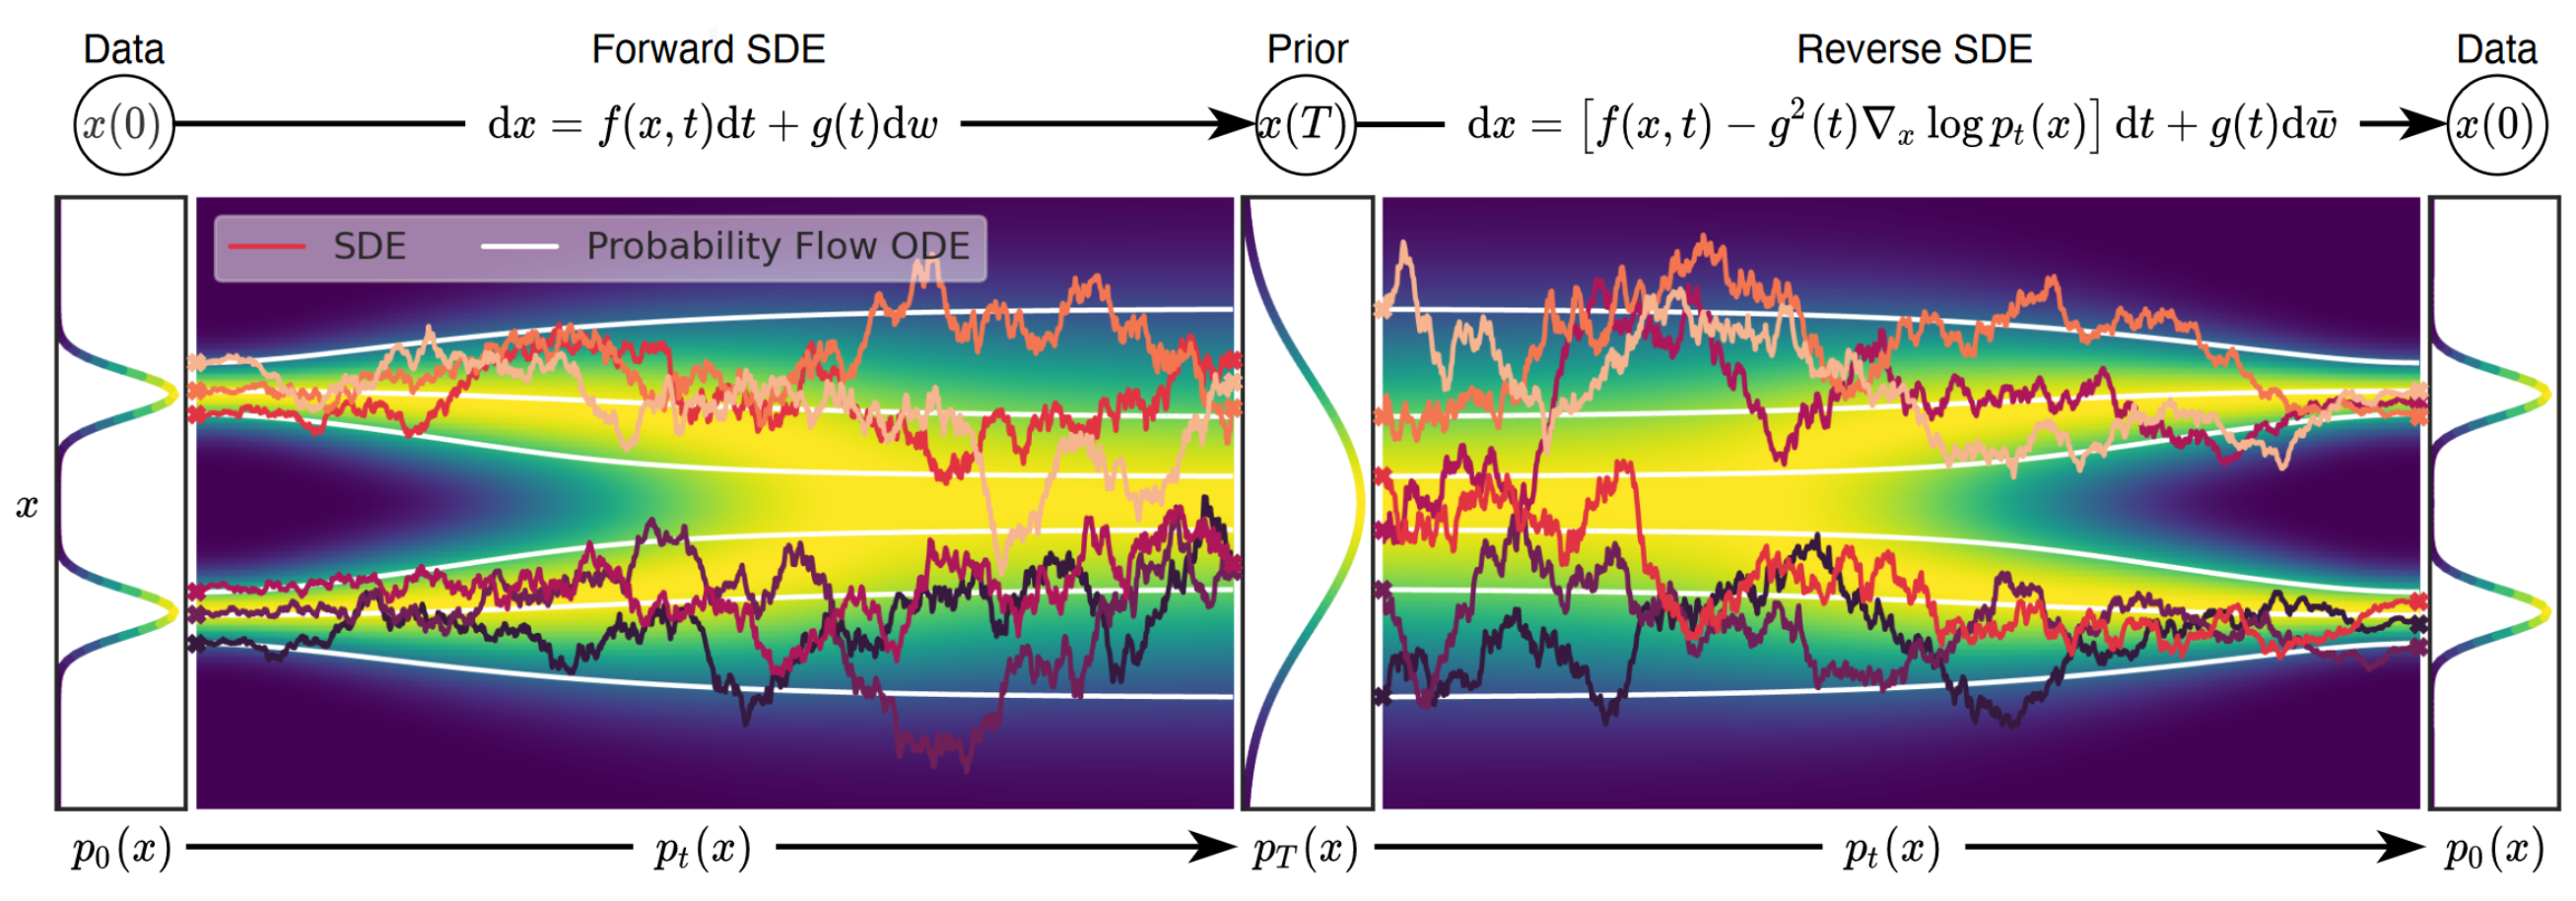
\includegraphics[width=1\columnwidth]{figures/DiffusionModels_SDEs.png}
    \caption{This figure, adapted from Song et al.~\citep{song2020score}, illustrates the two-fold process in score-based generative modeling through SDEs. On the left, the Forward SDE represents the gradual transformation of data into noise, guided by the drift and diffusion coefficients. On the right, the Reverse SDE depicts the process of reconstituting original data from noise, leveraging the known score of each marginal distribution.}\label{fig:DM_SDEs}
\end{figure}

Training a model to accurately estimate the score functions at various noise levels is a fundamental aspect of this process. To achieve this, the model is trained through score matching \citep{hyvarinenScoreMatching}, which involves fine-tuning the model to closely approximate these score functions across a spectrum of noise levels \citep{song2020score}. The training objective is to minimize the discrepancy between the estimated and true scores over time, influenced by the noise. The score matching process matches the output of the score network with the true gradient of the log-likelihood over the course of the SDE, enabling the generation of realistic data samples from complex distributions.